\documentclass[english,11pt]{beamer}

\DeclareMathOperator{\Cov}{Cov}
\DeclareMathOperator{\Var}{Var}
\DeclareMathOperator{\E}{\mathbb{E}}
\DeclareMathOperator{\Proba}{\mathbb{P}}

\newcommand{\Covb}[2]{\ensuremath{\Cov\!\left[#1,#2\right]}}
\newcommand{\Eb}[1]{\ensuremath{\E\!\left[#1\right]}}
\newcommand{\Pb}[1]{\ensuremath{\Proba\!\left[#1\right]}}
\newcommand{\Varb}[1]{\ensuremath{\Var\!\left[#1\right]}}

% norm
\newcommand{\norm}[1]{\| #1 \|}

\newcommand{\indep}{\rotatebox[origin=c]{90}{$\models$}}





\usepackage{mathptmx,amsmath,amssymb,graphicx,bibentry,bbm,babel,ragged2e}

\makeatletter

\newcommand{\noun}[1]{\textsc{#1}}
\newcommand{\jitem}[1]{\item \begin{justify} #1 \end{justify} \vfill{}}
\newcommand{\sframe}[2]{\frame{\frametitle{#1} #2}}

\newenvironment{centercolumns}{\begin{columns}[c]}{\end{columns}}
%\newenvironment{jitem}{\begin{justify}\begin{itemize}}{\end{itemize}\end{justify}}

\usetheme{Warsaw}
\setbeamertemplate{footline}[text line]{}
\setbeamercolor{structure}{fg=purple!50!blue, bg=purple!50!blue}

\setbeamersize{text margin left=15pt,text margin right=15pt}

\setbeamercovered{transparent}


\@ifundefined{showcaptionsetup}{}{%
 \PassOptionsToPackage{caption=false}{subfig}}
\usepackage{subfig}

\usepackage[utf8]{inputenc}
\usepackage[T1]{fontenc}



\makeatother

\begin{document}


\title{Invisible Bridges ? Scientific landscapes around similar objects studied from Economics and Geography perspectives}

\author{J.~Raimbault$^{1,2}$\\
\texttt{juste.raimbault@polytechnique.edu}
}


\institute{$^{1}$UMR CNRS 8504 G{\'e}ographie-cit{\'e}s\\
$^{2}$UMR-T IFSTTAR 9403 LVMT\\
}


\date{ECTQG 2017 - York\\\smallskip
Session 4A  - Bridges between Geography and Economics\\\smallskip
September 2017
}

\frame{\maketitle}





%%%%%%%%%%%%%%%%%%%
%% ABSTRACT
%\textbf{Keywords : } Quantitative Epistemology ; Citation Network ; Text Mining ; Bridges between Economics and Geography


% Titre : ref à Calvino, Invisible Cities ; here "potential" or "hidden" links, for example physics, or emerging subdisciplines, objects etc.




%%%%%%%%%%%%%%%%%
\section{Introduction}
%%%%%%%%%%%%%%%%%


\sframe{An Utopia of interdisciplinarity ?}{
\centering
\includegraphics[height=0.85\textheight]{figures/interdisc}

}




\sframe{Perspectivism}{

% Science in a perspectivist approach~(\cite{giere2010scientific}), it is natural and necessary that disciplines or fields propose very different \emph{perspectives} on real world objects. The yet-to-explore border regions at the interface, in which interdisciplinarity draws most of its strengths, are however not well understood in terms of processes of knowledge production such as domains cross-fertilisation, but also not necessarily the object of consensuses for research policies. 



\textit{Scientific Perspectivism~\cite{giere2010scientific} : each scientific entreprise as a perspective, which medium is called a model}


\bigskip

\textbf{Question 1 : } Which compromises between transversal approaches (interdisciplinary) and vertical approaches (specialization) ?

$\rightarrow$ Banos' virtual spiral~\cite{banos2013pour} ; Complex Systems integrated roadmap~\cite{2009arXiv0907.2221B}

\medskip

\textbf{Question 2 : } Taking interdisciplinarity as an objective, which processes of knowledge production and interactions between disciplines occur and would be desirable ?

}


\sframe{Geographical systems}{

\textit{Geographical System by essence heterogeneous and require interdisciplinarity}

\medskip

\cite{fujita1999evolution} : comparer à la théorie évolutive : juste reproduire hiérarchie, est-ce assez ? ; question de l'équilibre.

}


\sframe{Research Question}{

%We propose to explore these issues on the particular case of Economics and Geography, between which bridges seem difficult to build in the current state of disciplines.


\textbf{Research Objective}


}


\sframe{Methodology}{

% We take a Quantitative Epistemology approach, more precisely by combining citation network analysis with text-mining and semantic network analysis, using methods and tools developed in~\cite{raimbault2016indirect} to reconstruct what can be seen as a \emph{scientific landscape}. %As these are quite sensitive to context and choices to be made in exogenous delimitation of studied corpus, and as generality is not the best way to tackle epistemological questions,
% We choose to work on two case studies of objects that have been extensively studied from both perspectives: Relations between Network and Territories, and Urban Growth. We constitute for each an initial corpus of key references in both disciplines, from which the backward citation network at depth two is reconstructed. We then collect abstracts for a significant proportion of nodes, extract relevant keywords, and couple the citation network with a semantic network which communities for example define endogenous research domains.





}





%%%%%%%%%%%%%%%%%
\section{Case studies}
%%%%%%%%%%%%%%%%%


\sframe{Interactions between Networks and Territories}{

% intiail corpus
% ...

% Results overall show that as expected disciplines are highly clustered in terms of citation practice, but still form a fully connected graph. The communities correspond to clearly distinct contents in term of semantic landscape, with a good agreement between community structures in both networks. In the case of Network and Territories, intermediate or sub-disciplines emerge as communities in the citation network, as specializations on Accessibility or Transit-Oriented-Development that position at the interface of Planning, Geography and Economic Geography. Similarly, unexpected ``newcomers'' such as physicists appear at equal distance of Geography and Economics and may be an interesting direction to search for bridges.



}



\sframe{Citation Network}{
\centering
%\vspace{-0.5cm}
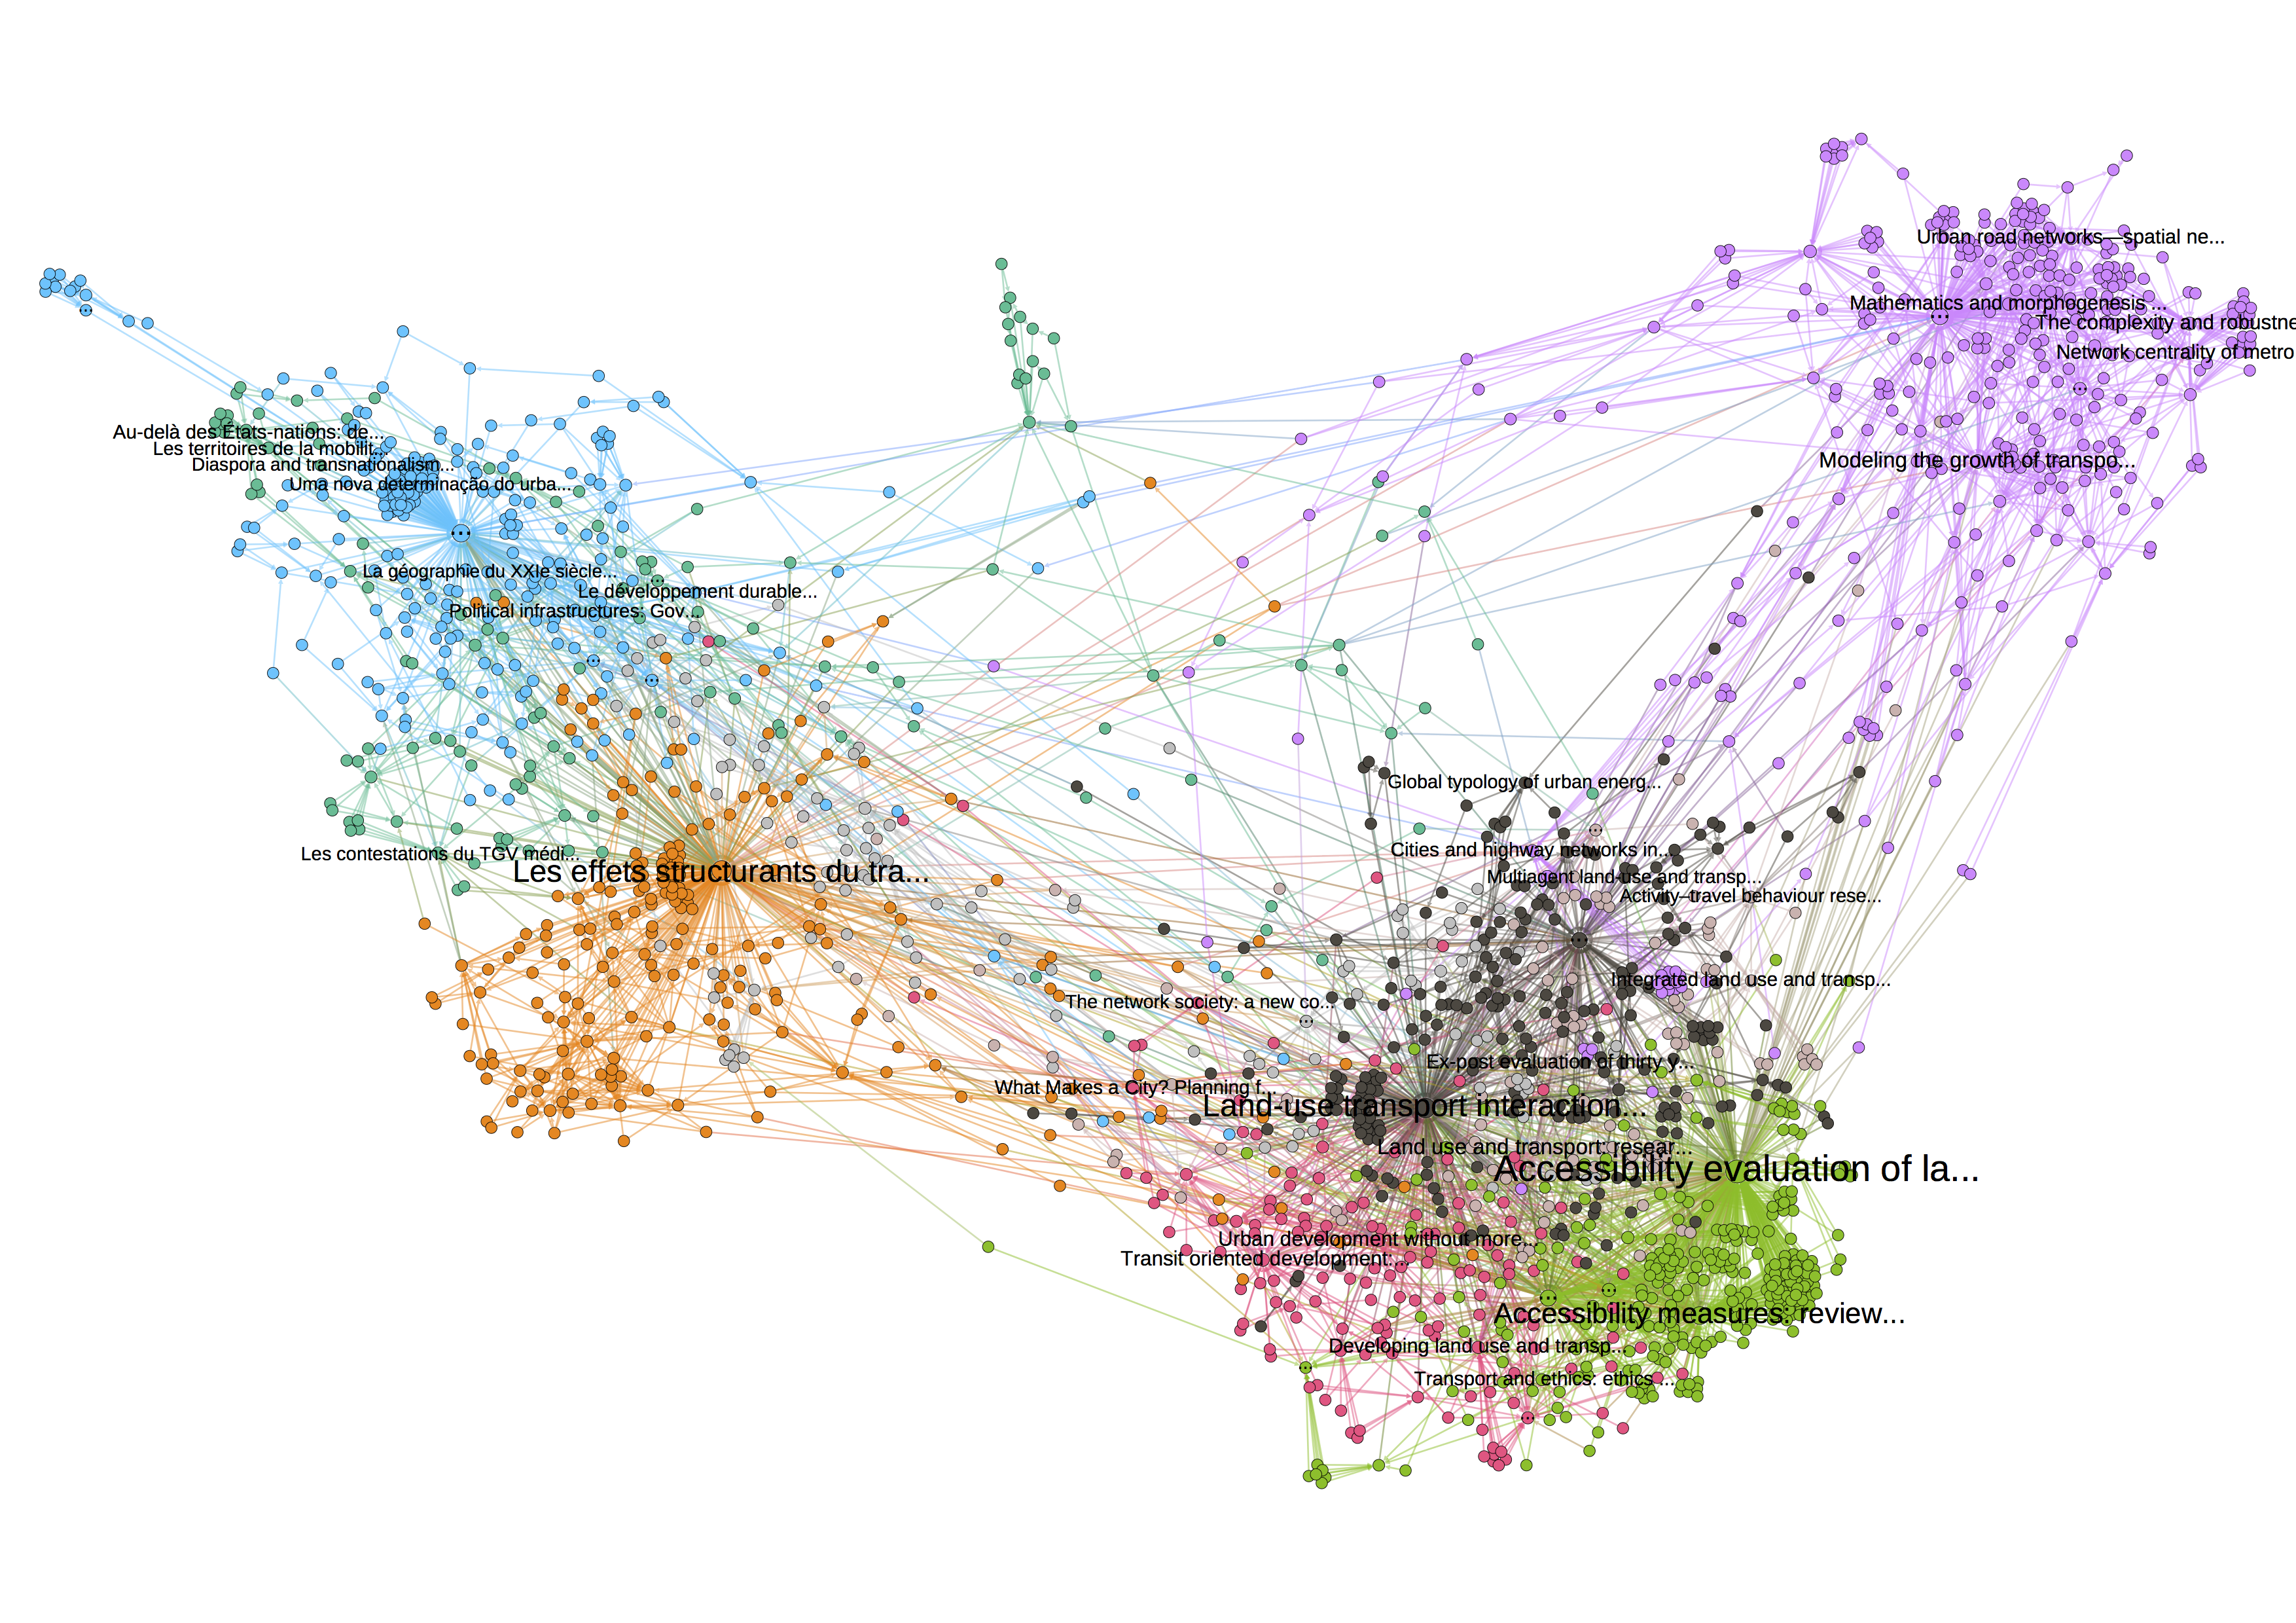
\includegraphics[height=0.9\textheight]{figures/rawcore}
}

\sframe{Citation Network Properties}{

}



\sframe{Semantic Network}{
\centering
%\vspace{-0.5cm}
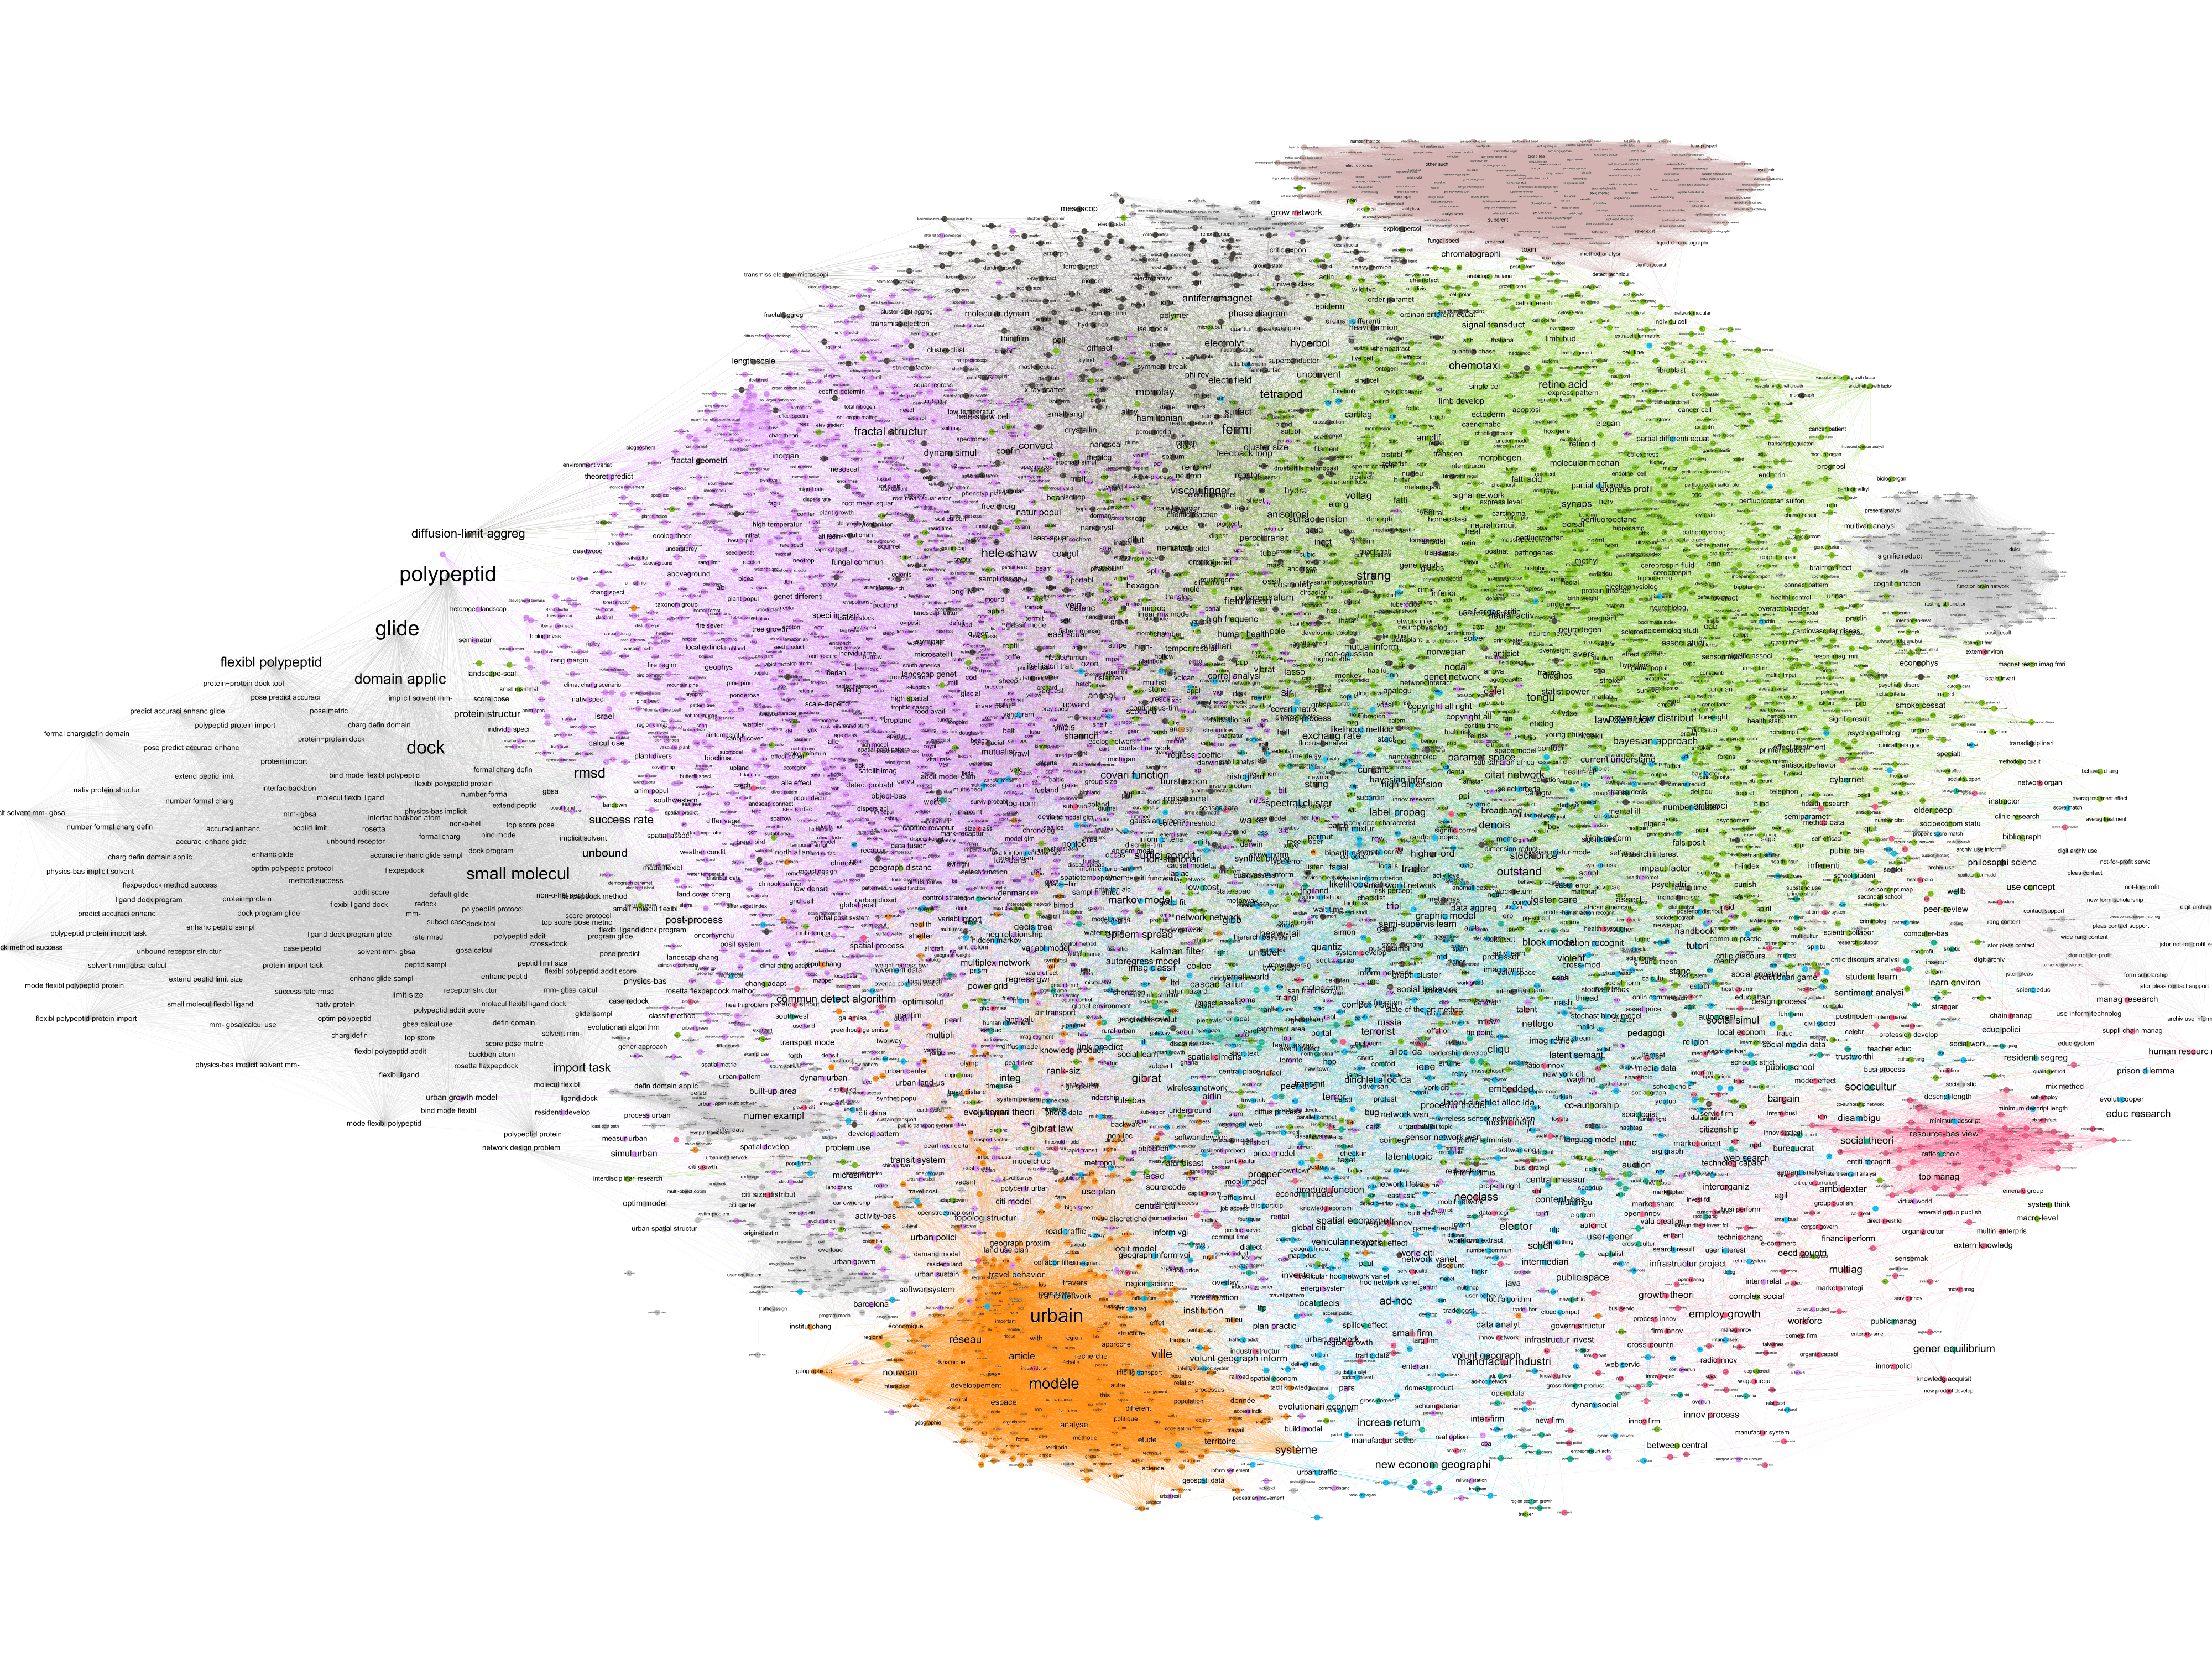
\includegraphics[height=\textheight]{figures/semantic}
}


\sframe{Semantic communities}{

\footnotesize
\vspace{-0.8cm}
\begin{table}
\label{tab:quantepistemo:semanticdomains}
\begin{tabular}{llll}
\hline\noalign{\smallskip}
Name & Size & Weight & Keywords  \\
\noalign{\smallskip}\hline\noalign{\smallskip}
Networks & 820 & 13.57\% & \texttt{social network, spatial network, resili} \\
Policy & 700 & 11.8\% & \texttt{actor, decision-mak, societi} \\
Socio-economic & 793 & 11.6\% & \texttt{neighborhood, incom, live} \\
High Speed Rail & 476 & 7.14\% & \texttt{high-spe, corridor, hsr} \\
French Geography & 210 & 6.08\% & \texttt{système, développement, territoire} \\
Education & 374 & 5.43\% & \texttt{school, student, collabor} \\
Climate Change & 411 & 5.42\% & \texttt{mitig, carbon, consumpt} \\
Remote Sensing & 405 & 4.65\% & \texttt{classif, detect, cover} \\
Sustainable Transport & 370 & 4.38\% & \texttt{sustain urban, travel demand, activity-bas} \\
Traffic & 368 & 4.23\% & \texttt{traffic congest, cbd, capit} \\
Maritime Networks & 402 & 4.2\% & \texttt{govern model, seaport, port author} \\
Environment & 289 & 3.79\% & \texttt{ecosystem servic, regul, settlement} \\
Accessibility & 260 & 3.23\% & \texttt{access measur, transport access, urban growth} \\
Agent-based Modeling & 192 & 3.18\% & \texttt{agent-bas, spread, heterogen} \\
Transportation planning & 192 & 3.18\% & \texttt{transport project, option, cba} \\
Mobility Data Mining & 168 & 2.49\% & \texttt{human mobil, movement, mobil phone} \\
Health Geography & 196 & 2.49\% & \texttt{healthcar, inequ, exclus} \\
Freight and Logistics & 239 & 2.06\% & \texttt{freight transport, citi logist, modal} \\
%Spanish Geography & 106 & 1.26\% & \texttt{movilidad urbana, criteria, para} \\
Measuring & 166 & 1.0\% & \texttt{score, sampl, metric} \\
\noalign{\smallskip}\hline
\end{tabular}
\end{table}
%%%%%%%%%%%%%%%%%%


}


\sframe{Interdisciplinarity patterns}{
\centering

\includegraphics[width=0.5\textwidth]{figures/interdisciplinarities}
\includegraphics[width=0.5\textwidth]{figures/compo_proportion}

\footnotesize

\textit{Distribution of interdiscplinarities (Left) and semantic composition of citation communities (Right)}
}

\sframe{Community Proximities}{
\centering

\includegraphics[width=0.5\textwidth]{figures/citation_proximities}
\includegraphics[width=0.5\textwidth]{figures/semantic_proximities}

\footnotesize

\textit{Proximities between citation communities (Left) and semantic communities (Right)}

}


\sframe{Urban growth}{

% description of content ?

% On the subject of Urban Growth, the distinctions are even stronger, with a final range of sub-disciplines spanning from technical GIS studies to entrepreneurship and ``creative clusters'' studies.

}


\sframe{Urban growth : Citation Network Structure}{

% modularity : 0.7011859
% bootstrap : 2.19881121709871e-05 +- 0.000781439698557175

% communities : '22'='Urban Ecology','8'='Urban Sociology','16'='Housing Market','5'='Spatial Statistics','19'='Economic Geography','23'='Criminology','1'='Cellular Automata','10'='Urban Simulation','9'='Development','2'='Ecology','20'='Mobility','6'='LUTI','4'='Networks','18'='Economy of Information'


}



%%%%%%%%%%%%%%%%%
\section{Discussion}
%%%%%%%%%%%%%%%%%

% This illustrates how each discipline has constructed its own objects and epistemologies, and how difficult it can be to actually work on a common object. It is interesting then to formulate assumptions on the role of auxiliary and neighbor disciplines in shaping research subjects of a given discipline, and in particular of performative branches that have rapid practical application (e.g. in socio-economic practices and policies for Economics, in Planning and Urbanism for Geography) that seem to simultaneously drive them apart but also bring new potential common objects (such as the ``smart city''). We postulate that bridging approaches are closer than they seem but that they will require a high level of reflexivity and awareness of scientific landscape as this example illustrates.



\sframe{Discussion}{

}




\sframe{Conclusion}{

\justify

$\rightarrow$ 

\bigskip
\bigskip
\bigskip


\footnotesize{ - Code et data available at\\ \texttt{https://github.com/JusteRaimbault}
}

}






\sframe{Reserve slides}{

\centering

\Large

\textbf{Reserve Slides}

}



\sframe{Measuring Interdisciplinarity}{
\begin{itemize}
\item References as probability matrix for themes $\mathbf{P}=(p_{ij})$~\cite{bergeaud2017classifying}
\item First order interdisciplinarity $I_i = 1 - \sum_j p_{ij}^2$
\item Let $\mathbf{A}$ citation network adjacency matrix, $\mathbf{I}_k$ row selection matrix for class $k$ ($Id\cdot \mathbbm{1}_{c(i)=k}$) such that $I_k \cdot A \cdot I_{k'}$ gives exactly citations from $k$ to $k'$
\item Citation proximity given by $c_{kk'} = \sum \mathbf{I}_k \cdot \mathbf{A} \cdot \mathbf{I}_{k'} /  \sum \mathbf{I}_k \cdot \mathbf{A}$
\item Semantic distance $\mathbf{D} = d_{ii'}=\sqrt{\frac{1}{2}\sum (p_{ij}-p{i'j})^2}$ and Semantic proximity given by $s_{kk'} = \mathbf{I}_k \cdot \mathbf{D} \cdot \mathbf{I}_{k'} / \sum \mathbf{I}_k \sum \mathbf{I}_{k'}$
\end{itemize}
}




%%%%%%%%%%%%%%%%%%%%%
\begin{frame}[allowframebreaks]
\frametitle{References}
\bibliographystyle{apalike}
\bibliography{/Users/Juste/ComplexSystems/CityNetwork/Biblio/Bibtex/CityNetwork}
\end{frame}
%%%%%%%%%%%%%%%%%%%%%%%%%%%%









\end{document}







